\documentclass[11pt]{beamer}

\usetheme{metropolis}
\usepackage{appendixnumberbeamer}

\usepackage{booktabs}
\usepackage[scale=2]{ccicons}

\usepackage{pgfplots}
\usepgfplotslibrary{dateplot}

\metroset{block=fill}
\usepackage{xspace}
\newcommand{\themename}{\textbf{\textsc{metropolis}}\xspace}

\usefonttheme[onlymath]{serif}
\usepackage{amsmath,amsthm}
\usepackage{graphicx} % Allows including images
\usepackage{booktabs} % Allows the use of \toprule, \midrule and \bottomrule in tables
%\newtheorem{lemma}[theorem]{Lemma}



%\usepackage[english]{babel}  % Show english numerate
%\usepackage{epsfig,amssymb,amsmath,version}
%\usepackage{amssymb,version,graphicx,fancybox,mathrsfs,multirow}
\usepackage{epstopdf}
\usepackage{url,hyperref}
%
%\usepackage{newtxtext}
\usepackage{color,xcolor}
%\usepackage{cases}
%\usepackage{mathtools}

%\setbeamerfont{normal text}{family=\songti}
%\setbeamerfont{frametitle}{family=\large\bfseries}
%\setbeamerfont{title}{family=\bfseries}
%\setbeamerfont{subtitle}{family=\kaishu}
%\setbeamerfont{institute}{size=\small}
\definecolor{iron}{RGB}{0,82,67}
\setbeamercolor{frametitle}{bg=iron}
%\setbeamercolor{progress bar}{fg=iron,bg=iron}

%\title{Metropolis}
%\subtitle{A modern beamer theme}
%\date{\today}
%\author{Matthias Vogelgesang}
%\institute{Center for modern beamer themes}

\title[Short title]{Full Title of the Talk}
\subtitle{A modern beamer theme}
\author{Matthias Vogelgesang} % Your name
\institute{Center for modern beamer themes \\ % Your institution for the title page
%\medskip
%\textit{john@smith.com} % Your email address
}
\date{\today} % Date, can be changed to a custom date


\graphicspath{{./Figures/}}

% \titlegraphic{\hfill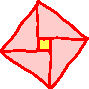
\includegraphics[height=1.5cm]{logo.pdf}}

\begin{document}

\maketitle

\begin{frame}{Table of contents}
  %\bfseries
  \setbeamertemplate{section in toc}[sections numbered]
  \tableofcontents[hideallsubsections]
\end{frame}


%----------------------------------------------------------------------------------------
%	PRESENTATION SLIDES
%----------------------------------------------------------------------------------------

%------------------------------------------------
\section{First Section} % Sections can be created in order to organize your presentation into discrete blocks, all sections and subsections are automatically printed in the table of contents as an overview of the talk
%------------------------------------------------

\subsection{Subsection Example} % A subsection can be created just before a set of slides with a common theme to further break down your presentation into chunks

\begin{frame}
\frametitle{Paragraphs of Text}
This is paragraphs of text. The quick brown fox jumps over the lazy dog. The quick brown fox jumps over the lazy dog. The quick brown fox jumps over the lazy dog. The quick brown fox jumps over the lazy dog. The quick brown fox jumps over the lazy dog. \\~\\

The quick brown fox jumps over the lazy dog. The quick brown fox jumps over the lazy dog. The quick brown fox jumps over the lazy dog. The quick brown fox jumps over the lazy dog. The quick brown fox jumps over the lazy dog. The quick brown fox jumps over the lazy dog. The quick brown fox jumps over the lazy dog. The quick brown fox jumps over the lazy dog.
\end{frame}

%------------------------------------------------

\begin{frame}
\frametitle{Lists}

\begin{enumerate}
  \item This is a enumerate environment.
  \item This is a enumerate environment.
  \item This is a enumerate environment.
\end{enumerate}

\vspace{2ex}
\begin{itemize}[<+-| alert@+>]
\item This is a itemize environment.
\item This is a itemize environment.
\item This is a itemize environment.
\end{itemize}
\end{frame}

%------------------------------------------------

\begin{frame}
\frametitle{Blocks of Highlighted Text}
\begin{block}{Block Title}
This is the block environment. The quick brown fox jumps over the lazy dog. The quick brown fox jumps over the lazy dog. The quick brown fox jumps over the lazy dog.
\end{block}

\begin{exampleblock}{Block Title}
This is the exampleblock environment. The quick brown fox jumps over the lazy dog. The quick brown fox jumps over the lazy dog.
\end{exampleblock}

\begin{alertblock}{Block Title}
This is the alertblock environment. The quick brown fox jumps over the lazy dog. The quick brown fox jumps over the lazy dog.
\end{alertblock}
\end{frame}

%------------------------------------------------

\begin{frame}
\frametitle{Multiple Columns}
\begin{columns}[c] % The "c" option specifies centered vertical alignment while the "t" option is used for top vertical alignment

\column{0.5\textwidth}
This is a text in first column.
$$E=mc^2$$
\begin{itemize}
\item First item
\item Second item
\end{itemize}

\column{0.5\textwidth}
This text will be in the second column
and on a second tought this is a nice looking
layout in some cases.

\end{columns}
\end{frame}

%------------------------------------------------
\section{Second Section}
%------------------------------------------------

\begin{frame}
\frametitle{Table and Lemma}
\begin{table}
\caption{Table caption}
\begin{tabular}{l l l}
\toprule
Treatments & Response 1 & Response 2 \\
\midrule
Treatment 1 & 0.0003262 & 0.562 \\
Treatment 2 & 0.0015681 & 0.910 \\
Treatment 3 & 0.0009271 & 0.296 \\
\bottomrule
\end{tabular}
\end{table}

\begin{lemma}
This is a lemma environment.
\end{lemma}
\end{frame}


%------------------------------------------------


\begin{frame}[fragile] % Need to use the fragile option when verbatim is used in the slide
\frametitle{Verbatim}
\begin{example}[Theorem Slide Code]
\begin{verbatim}
\begin{frame}
\frametitle{Theorem}
\begin{theorem}[Mass--energy equivalence]
$E = mc^2$
\end{theorem}
\end{frame}\end{verbatim}
\end{example}

\begin{theorem}[Mass--energy equivalence]
$E = mc^2$
\end{theorem}
\end{frame}

%------------------------------------------------

\begin{frame}
\frametitle{Figure}

Uncomment the code on this slide to include your own image from the same directory as the template .TeX file.
\begin{figure}[htp!]
\centering
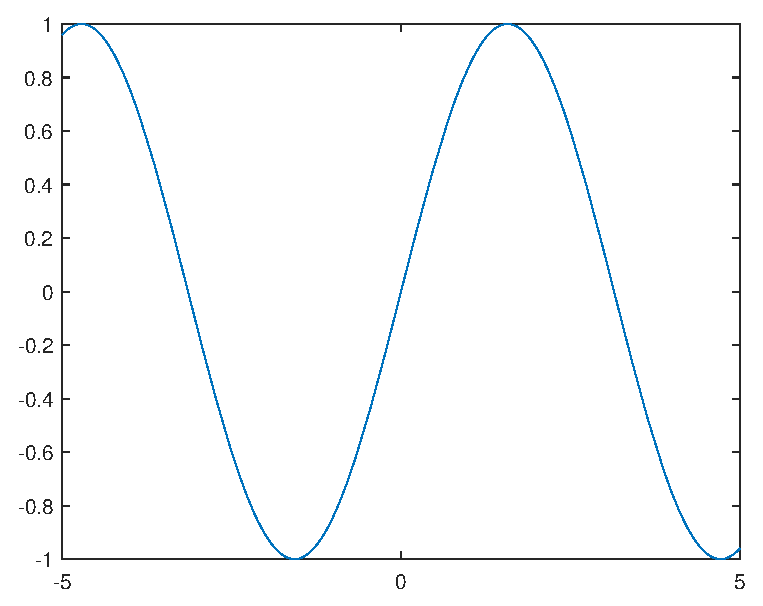
\includegraphics[width=0.6\linewidth]{Image.eps}
\end{figure}
\end{frame}

%------------------------------------------------

\begin{frame}[fragile] % Need to use the fragile option when verbatim is used in the slide
\frametitle{Citation}
An example of the \verb|\cite| command to cite within the presentation:\\~

This statement requires citation \cite{Smith2012}.
\end{frame}

%------------------------------------------------

\begin{frame}
\frametitle{References}
\footnotesize{
\begin{thebibliography}{99} % Beamer does not support BibTeX so references must be inserted manually as below
\bibitem[Smith, 2012]{Smith2012} John Smith. Title of the publication. \emph{Journal Name}, 12(3):45--678, 2012.
\end{thebibliography}
}
\end{frame}




\begin{frame}[standout]
  \Huge Thank you!
\end{frame}



%\begin{frame}[standout]
%  Questions?
%\end{frame}

%\appendix

%\begin{frame}[fragile]{Backup slides}
%  Sometimes, it is useful to add slides at the end of your presentation to
%  refer to during audience questions.
%
%  The best way to do this is to include the \verb|appendixnumberbeamer|
%  package in your preamble and call \verb|\appendix| before your backup slides.
%
%  \themename will automatically turn off slide numbering and progress bars for
%  slides in the appendix.
%\end{frame}

%\begin{frame}[allowframebreaks]{References}
%
%  \bibliography{demo}
%  \bibliographystyle{abbrv}
%
%\end{frame}

\end{document}
